\documentclass[a4paper,12pt]{article}

\usepackage{url}
\usepackage{epsfig}
\usepackage{graphics}
\usepackage{fancyhdr}
\usepackage{amsmath}
\usepackage{array,xcolor,colortbl}
\usepackage{multirow}
\usepackage{multicol}
\usepackage{float}
\usepackage{adjustbox}
\usepackage{enumitem}
\usepackage{caption}
\usepackage{subcaption}
\usepackage{tablefootnote}


\graphicspath{{pictures/}}

\title{Report Assignment 2 DD2380}
\author{\hspace*{-0.5cm}
GROUP 2:26\\
\begin{tabular}{cccc}
Vilmer Jonsson \\
2001-06-26  \\
vilmerj@kth.se \\
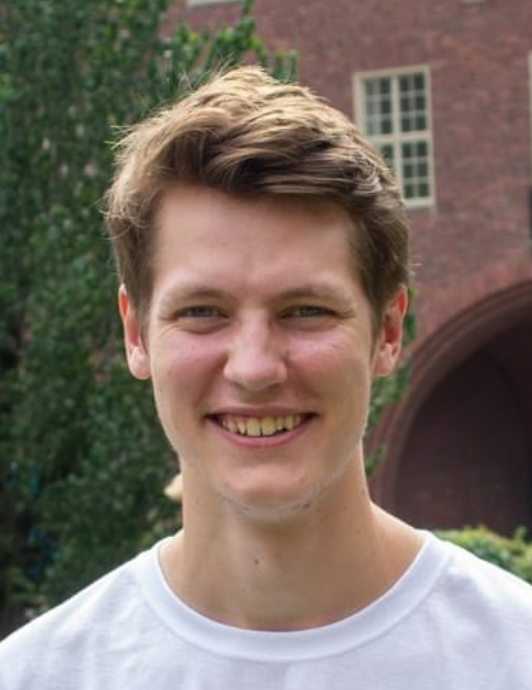
\includegraphics[width=0.13\linewidth]{Vilmer_Jonsson.jpg}
\end{tabular}} 
% Normally there will not be any pictures but we want
% these so that we can connect faces to names in the course
% We also want birthdates so that we can tell people with the same
% name apart
\date{\today}

\pagestyle{fancy}
\setlength{\headheight}{15pt}
\fancyhf{}
\lhead{DD2438} % DO NOT REMOVE!!!!
\rhead{Vilmer Jonsson} %% UPDATE WITH YOUR NAMES
\fancyfoot[C, CO]{\thepage}

\begin{document}

\maketitle
\thispagestyle{fancy}

\begin{abstract}

When several vehicles are maneuvering in the same area, it is important to be able to predict the future behavior of the other vehicles. This report presents a solution to two problems. Firstly, the traffic problem, where each vehicle is trying to reach its goal as fast as possible. Secondly, the formation problem, where several vehicles are trying to reach targets in a coordinated manner. The solution to the traffic problem is based on velocity obstacles, individual path planning and recalculating the path when needed. The solution to the formation problem is based on adjusting the velocity of the vehicles to reach the goal at the same time. The results show that the implementation works well. Two of the 16 tests were not completed, both of these had problems with cars merging. The best group had a similar approach to the formation problem but a slightly different approach to the traffic problem.



\end{abstract}


\clearpage

\begin{multicols}{2}

%%%%%%%%%%%%%%%%%%%%%%%%%%%%%%%%%%%%%%%%%%%%%%%%%%%%%%%%%%%%%
%%%%%%%%%%%%%%%%%%%%%%%%%%%%%%%%%%%%%%%%%%%%%%%%%%%%%%%%%%%%%
\section{Introduction}
\label{sec:intro}

When maneuvering a vehicle, there is often several other vehicles in the vicinity. These vehicles are maneuvered by other drivers, who all have their own goals and intentions. To be able to maneuver a vehicle safely, it is important to be able to predict the future behavior of these other vehicles. When driving a car, this is done by the driver, who uses his or hers knowledge of the traffic rules and experience to predict the future behavior of the other vehicles. Logically, if you were to construct a self-driving car, you would need a similar system to predict the future behavior of the other vehicles and to be able to make decisions based on this information. 

This is one of the problems that this report will address. The other problem is similar, but instead of the vehicles trying to get to separate goals independently, they are trying to reach several close targets in a coordinated manner. The first problem will be called the \emph{Traffic} problem and the second problem will be called the \emph{Formation} problem.

The most important part of the solution to the Traffic problem is to be able to predict the future behavior of the other vehicles. This is done by using the concept of velocity obstacles. Velocity obstacles are a way of predicting whether a certain velocity will result in a collision with another vehicle. This was used since it is a simple and efficient way of ensuring that no collisions will occur.

The most important part of the solution to the Formation problem is to be able to get the vehicles to adjust their velocity to reach targets at the same time. The solution is based on a leader-follower approach, where one vehicle is the leader and the other vehicles try to keep a certain distance to the leader.



\subsection{Contribution}
In this project, a solution to the Traffic problem using velocity obstacles, individual path planning and recalculating the path when needed. For the Formation problem, the contribution is a method to get the vehicles to follow their individual paths and adjust their velocity to reach the goal in a coordinated manner.

\subsection{Outline}
In section \ref{sec:relwork}, related work to both the Traffic and Formation problem will be introduced in order to give the reader more information about the past research in the area. In section \ref{sec:method}, the implementation will be presented in more detail. In section \ref{sec:exps}, the experimental results will be presented and analyzed based on the best group's performance.

%%%%%%%%%%%%%%%%%%%%%%%%%%%%%%%%%%%%%%%%%%%%%%%%%%%%%%%%%%%%%
%%%%%%%%%%%%%%%%%%%%%%%%%%%%%%%%%%%%%%%%%%%%%%%%%%%%%%%%%%%%%
\section{Related work}
\label{sec:relwork}
% \emph{Related Work section describing and referring to at least 5 research papers}

Avoiding other vehicles is a problem as old as traffic itself. However, in robotics the development were first done on trying to collide with objects. One of the first use-cases was a missile trying to hit a moving target. This was done by using the relative velocity of the missile and the target to calculate the optimal path for the missile. \cite{adler1956missile}

\begin{figure}[H]
  \centering
  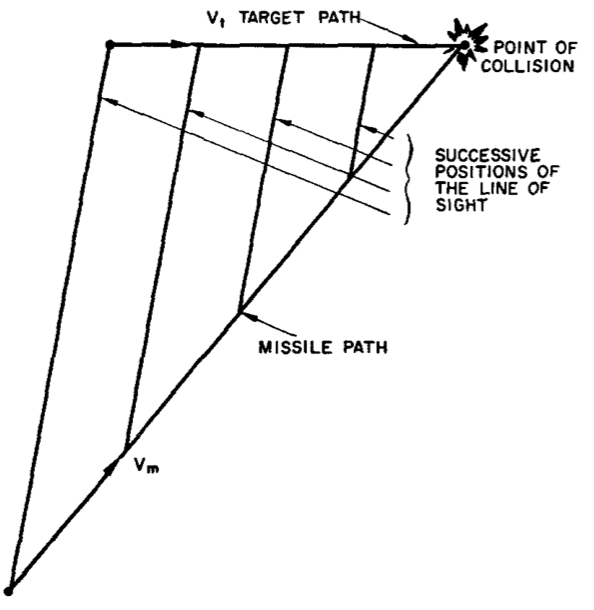
\includegraphics[width=0.45\textwidth]{missile.png}
  \caption{Proportional navigation, a method used to calculate the optimal path for a missile to hit a moving target. \cite{adler1956missile}}
  \label{fig:missile}
\end{figure}

Velocity obstacles were first introduced by Fiorini and Shiller in 1998. They are a way of predicting whether a certain velocity will result in a collision with another vehicle. This is done by defining a cone which has one tip in the center of the vehicle and intersects with the other vehicle on the boundary of the cone. The whole cone is then moved along the velocity vector of the other vehicle. If the cone intersects with the vehicles' velocity vector, the velocity is not safe. \cite{doi:10.1177/027836499801700706}

\begin{figure}[H]
  \centering
  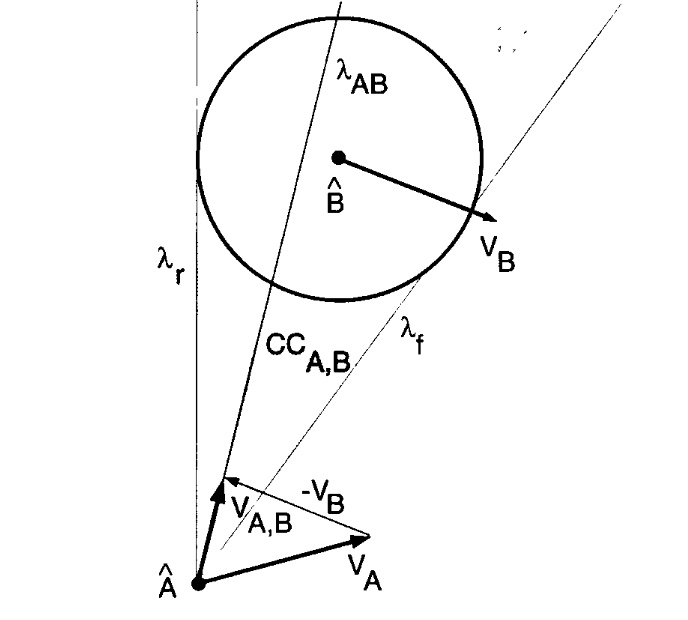
\includegraphics[width=0.45\textwidth]{velObstacles.jpg}
  \caption{Velocity obstacles. The circle is the moving obstacle and the vehicles current position is A. \cite{doi:10.1177/027836499801700706}}
  \label{fig:velObstacles}
\end{figure}

A development to velocity obstacles called \emph{Reciprocal Velocity Obstacles} were introduced in 2008 by van den Berg et al. This method is more efficient than velocity obstacles since it assumes that the other vehicle is also trying to avoid a collision. This means that both vehicles will try to avoid each other and do not have to steer away as much as with traditional velocity obstacles. It also avoids the problem of oscillations that can occur with traditional velocity obstacles, see Figure~\ref{fig:reciprocal}.
\cite{van2008reciprocal}

\begin{figure}[H]
  \centering
  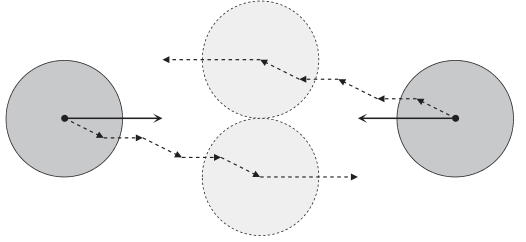
\includegraphics[width=0.45\textwidth]{reciprocal.jpg}
  \caption{Oscillations when two agents avoid each other using traditional velocity obstacles. \cite{van2008reciprocal}}
  \label{fig:reciprocal}
\end{figure}

The same authors to the previous paper also introduced a method called Hybrid Reciprocal Velocity Obstacles in 2011. The difference to reciprocal velocity obstacles is that the vehicles are encouraged to pass each other on the same side. If the vehicle needs to go on the other side, it will give full priority to the other vehicle. This is done in order to avoid the agents "dancing" around each other since they can not decide which side to pass on. \cite{snape2011hybrid}

For formation keeping, one method is the leader-follower approach. This means that one vehicle is the leader and the other vehicles are followers. The followers then adjust their velocity to keep a certain distance to the leader. The leader gets input from an external source while the followers get input from the leader. This is a simple and efficient way of keeping formation. There is no feedback to the leader from the followers. \cite{9214872}


%%%%%%%%%%%%%%%%%%%%%%%%%%%%%%%%%%%%%%%%%%%%%%%%%%%%%%%%%%%%%
%%%%%%%%%%%%%%%%%%%%%%%%%%%%%%%%%%%%%%%%%%%%%%%%%%%%%%%%%%%%%
\section{Proposed method}
\label{sec:method}
\emph{Proposed Method section explaining what you did in more detail. Use references and explain how you adapt, build upon, or use elements of the algorithms proposed in the reference.}

\subsection*{Traffic problem}

The solution to the traffic problems rely heavily on the concept of velocity obstacles. Each agent is first assigned a path based on an A* algorithm on a visibility graph. The paths consist of several numbered checkpoints that the agent should pass in order to not collide with static obstacles, for example walls.

The agents begin to move along their paths and at each time step, they calculate the velocity obstacles for neighboring agents. If the agent is in a collision course with another agent, it will sample close velocities and choose the one that is closest to the desired velocity and does not result in a collision. If none of the sampled velocities are safe, the agent will take the "least unsafe" velocity.

\subsubsection*{Skipping checkpoints}
The path finding algorithm will return the shortest path between the start and the goal. However, this path might not be the shortest if the agent is straying from the path. To avoid this, the agent will skip checkpoints if it is safe to do so. This is done by checking if there is a static obstacle between the agent and the next checkpoint. If there is not, the agent will skip the checkpoint and move towards the next one. This is checked at each time step.

\subsubsection*{Recalculating paths}
The agent will always try to move towards the next checkpoint. However, if there is a static obstacle in the way, the agent will not be able to reach the checkpoint. In this case, the agent will recalculate the path to the goal and thus avoid the obstacle. This is done by using the A* algorithm on the visibility graph again.


\subsubsection*{Recovering}
Recovering from crashes are an important part of the system. If an agent is in a crash, it will try to recover by moving backwards and turning at full steering angle. This is done to avoid getting stuck in a corner or similar. This method is not optimal and would need to be improved in order to work properly.

\subsection*{Formation problem}
The formation problem is solved by using something similar to leader-follower but much simpler since the performance is only measured by two factors:
\begin{itemize}
    \item The time of the last agent to reach the goal.
    \item The difference in time between the first and last agent to reach each checkpoint.
\end{itemize}

This means that the formation does not have to be perfect at all times, only at the checkpoints. The agents will adjust their velocity to reach the checkpoints at the same time. This is done by calculating the distance to the next checkpoint for every agent and adjusting the velocity based on the ratio defined in equation~\ref{eq:ratio}.

\begin{equation} \label{eq:ratio}
  \frac{\text{distance to checkpoint}}{\text{greatest distance to checkpoint}}
\end{equation}

If the greatest distance to the checkpoint is close to zero, the agent will adjust its velocity to reach the checkpoint as fast as possible. Note that the ratio is not used directly to scale the velocity linearly, but rather to determine whether the agent should speed up or slow down. If the ratio less than a certain threshold, the agent will stop and wait for the other agents to catch up.

Ideally, the agents should avoid each other similar to the traffic problem. However, this was not implemented due to time constraints. This was not needed for the tests that were performed, but would be needed in a more complex environment. The reason for it not being needed in the tests is that the agents do not hold formation at all times, only at the checkpoints. This means that the agents often will be far apart and not in danger of colliding with each other.


\subsection{Implementation}
\label{sec:impl}


\subsubsection*{Neighbors}
One part of the implementation is to determine which agents are neighbors to the agent. This is done by checking the distance between the agents. If the distance is less than a certain threshold, the agent is considered a neighbor. The threshold is dynamic and increases with the velocity of the agent. An agent is also considered a neighbor if the two agent's displacement vectors, \( \vec{v}_A + \vec{pos}_A \), are at a certain distance from each other. This is done since these agents will collide head on if they continue on their current paths.


\subsubsection*{Sample velocities}
The car will sample velocities in an arc in front of it. The arc is defined by the maximum turning angle of the car, the distance between the arc and the car are defined by the current velocity of the car.

The drone will sample velocities based on acceleration. This is done since the drone takes two accelerations, lateral and longitudinal, as input commands. The drone will sample accelerations in a circle around the current velocity of the drone. The radius of the circle is defined by the maximum acceleration of the drone. The resulting velocities are calculated by equation~\ref{eq:sample}. If the sampled velocity's magnitude is greater than the maximum velocity of the drone, it will be scaled down to the maximum velocity. Note that this is a simplification of acceleration's effect on velocity.

\begin{equation} \label{eq:sample}
    v_{new} = v_{current} + 0.5a
\end{equation}

The sampled velocities are sorted based on the distance to the desired velocity. The velocity that is closest to the desired velocity and does not result in a collision is chosen. Naturally, if two agents head right towards each other, they will both choose to pass each other on the same side, exactly as hybrid velocity obstacles.


\subsubsection*{Least unsafe velocity}  % Maybe move to implementation
Determining the least unsafe velocity when none of the sampled velocities are safe is done by a simple heuristic. Every sampled velocity is tested on all velocity obstacles until it finds an obstacle it is colliding with.


\subsubsection*{Performance issues}
Since velocity obstacles, checkpoint skipping and path recalculating are all computed after start, the performance of the system is crucial to prevent lag. Some things done to improve performance is to only calculate velocity obstacles for neighbors the neighboring agents, sample velocities only if the agent is in a collision course with another agent and not check all sampled velocities if one is found to be safe.




% Some things done to improve performance. For example, only calculate velocity obstacles for neighbors within a certain distance. And only sample velocities if the agent is in a collision course with another agent. 

% Recalculate path if there is a static obstacle in the way is a problem. 



%%%%%%%%%%%%%%%%%%%%%%%%%%%%%%%%%%%%%%%%%%%%%%%%%%%%%%%%%%%%%
%%%%%%%%%%%%%%%%%%%%%%%%%%%%%%%%%%%%%%%%%%%%%%%%%%%%%%%%%%%%%
\section{Experimental results}
\label{sec:exps}
% \emph{Experimental Results section, containing results of other groups in a table, and analysis of the results. Why was method X best?}
% -\tablefootnote{No completion, counts as 2000 seconds.}


\end{multicols}
\newpage
\begin{table}[t]
\caption{Results on traffic problem for car and drone compared to the best time.}
\label{tab:trafficTimes}
\small
\makebox[\textwidth][c]{
\begin{tabular}{c|c|c|c|c|c|c|c|c|c|c} \hline
\multicolumn{1}{c}{Vehicle} & \multicolumn{5}{|c|}{Car}          & \multicolumn{5}{c}{Drone}         \\ \hline
Map                         & open    & semi open    & intersection    & highway    & onramp   & open    & semi open    & intersection    & highway    & onramp    \\ \hline
My time                    & 22.9 & 42.7 & 88.1 & -\tablefootnote{No completion, counts as 2000 seconds.} & -$^1$ & 17.62 & 21.4 & 31 & 41.6 & 41.82   \\ \hline
Best time                   & 18.98 & 22.6 & 50.1 & 65.62 & 43.34 & 17.62 & 18.74 & 29.22 & 41.02 & 41.82 \\ \hline
Best group                  & 3 & 3 & 11 & 2 & 25 & 26 & 7 & 27 & 25 & 26   
\end{tabular}
}
\end{table}
\begin{table}[t]
  \caption{Results on formation problem for car and drone compared to the best time.}
  \label{tab:formationTimes}
  \small
  \makebox[\textwidth][c]{
  \begin{tabular}{c|c|c|c|c} \hline
  \multicolumn{1}{c}{Vehicle} & \multicolumn{2}{|c|}{Car}          & \multicolumn{2}{c}{Drone}         \\ \hline
  Map                         & 6    & 6B    & 6    & 6B    \\ \hline
  My time                    & 93.25 & 94.38 & 109.18 & 66.58   \\ \hline
  Best time                   & 90.28 & 67.53 & 84.96 & 64.2\\ \hline
  Best group                  & 2 & 6 & 11 & 7  
  \end{tabular}
  }
  \end{table}


\begin{multicols}{2}






\subsection{Analysis of Outcome}

\begin{table}
\begin{center}
\begin{tabular}{|c|c|c|}
\hline
 & Problem A & Problem X \\ \hline
Group 1 & 100 & \bf45 \\ \hline
Group 2  & \bf42 & 66 \\ \hline
\end{tabular}
\caption{Group 1 performed better at Problem X and Group 2 performed better at Problem A.}
\label{tab:results}
\end{center}
\end{table}

The outcome of the final tests can be seen in Table~\ref{tab:trafficTimes} and Table~\ref{tab:formationTimes}. The results show that the drone performed better than the car in both the traffic and formation problem. The main reason for this is probably that while the car is faster than the drone, it is also larger and is affected more by crashes. The drone is also more agile and can steer in all directions, while the car's steering model is more limited. 

The results also show that my implementation was the best at two of the maps and often is very close to the best time, especially in the drone traffic problem. This is a good result and shows that the implementation is working well, but there is still room for improvement. Two of the maps were not completed, the highway and on-ramp maps for the car.

The best performing group was group 2. For the traffic problem, they relied a bit more on a dynamic path planning where they iterated over the paths and weighted the different nodes based on how many other cars pass that same node. That seems like a good idea and would probably decrease the number of crashes. For the formation problem, they had a similar approach to mine, but they only switched leader between the agents at the checkpoints. I think my approach is better since it is more flexible and does not rely on the agents being in a certain order. However, other parts of their implementation might have been better than mine, for example, they used a grid for their A* algorithm which ensures that the paths never collide with each other.

The fact that two maps were not completed should be seen as a failure. However, since I worked alone and thus had half the time to work on the project, I will not include an analysis of failure. However, I think that one of my problems was that the recovery mechanism was not good enough. The car often got stuck in corners and could not recover. Another problem is that the cars should slow down and form a queue when merging. Discover merging situations could be done by checking if the velocity vectors of the vehicles interfere with each other. The problem could also be solved by sampling velocities that are closer to the vehicle as well, and braking if they are free. For the car, the collision avoidance only sample velocities based on a different turn radius, not on braking or acceleration.

It should also be said that collisions did occur in my solution. This is not optimal and should be avoided. This makes the car drive into each other and slows them down or makes them stuck. This could be solved by sampling velocities that are closer to the vehicle as well, and braking if they are free.


%%%%%%%%%%%%%%%%%%%%%%%%%%%%%%%%%%%%%%%%%%%%%%%%%%%%%%%%%%%%%
%%%%%%%%%%%%%%%%%%%%%%%%%%%%%%%%%%%%%%%%%%%%%%%%%%%%%%%%%%%%%
\section{Summary and Conclusions}
\label{sec:summary}

The goal of this project was to implement solutions to the traffic and formation problems. For the traffic problem, the solution was to use velocity obstacles to avoid collisions with other agents. For the formation problem, the solution was to adjust the velocity of the agents to reach the goal at the same time. The results show that the drone performed better than the car in both problems. The implementation was close to the best time in most cases, but two maps were not completed. The best group was group 2, who had a similar approach to the formation problem but a slightly different approach to the traffic problem. The implementation failed on two of the maps for the car problem. Both of these maps were based on merging. A more sophisticated strategy for these scenarios would be needed to complete these maps.

The formation problem was not as complex as the traffic problem. The agents only had to reach the checkpoints at the same time, not hold formation at all times. However, in a real-life scenario where the agents would have to hold formation at all times, the formation problem would be much harder to solve. 


%%%%%%%%%%%%%%%%%%%%%%%%%%%%%%%%%%%%%%%%%%%%%%%%%%%%%%%%%%%%%
%%%%%%%%%%%%%%%%%%%%%%%%%%%%%%%%%%%%%%%%%%%%%%%%%%%%%%%%%%%%%
\end{multicols}
\clearpage
\bibliographystyle{plain}
\bibliography{reflist}


\end{document}
